\chapter{扰动场协同优化}

\section{扰动场谱分析}
我们首先确定工作在平衡场的本征坐标下 $\left(s, \theta^{*}, \varphi\right),$ 其中 $s \equiv \psi^{1 / 2}(\psi$ 是归一化极向磁通,充当径向坐标,磁面被定义为 $s$ 为常数的一个闭合面,特别的 $s=0$ 代表磁轴而 $s=1$ 表示等离子体边界, 另外取$\theta$ 到 $\theta^{*}(\theta)$ 的非线性变换使得磁力线在 $\left(s, \theta^{*}, \varphi\right)$ 坐标系统中是直线,即 $\left.\frac{d \varphi}{d \theta^{*}}\right|_{F L}=q$,下标 FL 表示取沿着磁力线方向的导数,接着定义三个方向的磁场分量:
% We work in the intrinsic equilibrium coordinates $\left(s, \theta^{*}, \varphi\right),$ where $s \equiv \psi^{1 / 2}(\psi$ being the normalized poloidal magnetic flux, cf. introduction) is used as a radial coordinate (in the $\left(s, \theta^{*}, \varphi\right)$ system of coordinates, a flux surface is defined by $s=c t e,$ in particular $s=0$ for the magnetic axis and $s=1$ for the separatrix $^{1}$ ), and $\theta^{*}$ is such that field lines are straight in the $\left(s, \theta^{*}, \varphi\right)$ system of coordinates:
% where the derivative is taken along a field line. We define:
\begin{equation}
B^{1} \equiv \vec{B} \cdot \vec{\nabla} s, \quad
B^{2} \equiv \vec{B} \cdot \vec{\nabla} \theta^{*}, \quad
B^{3} \equiv \vec{B} \cdot \vec{\nabla} \varphi
\label{de:B-comp}
% \tag{B^{i} \text{分量定义}}
\end{equation}

下面我们用磁场环向分量除以径向分量,该量最终会出现在磁岛半径计算的表达式中,此后我们对其进行 Fourier 分析找到与其所在有有理面共振的分量。
\begin{equation}
  \tilde{b}^{1} \equiv B^{1} / B^{3}
\end{equation}

% 而垂直磁面的归一化磁扰动分量有下面的表达式:
% and our radial-like normalized magnetic perturbations have the following expression:
% \[
% b^{r} \equiv \frac{b^{1}}{\sqrt{g^{11}}}
% \]

\begin{equation}
  \tilde{b}_{m n}^{1}(s) \equiv \int_{\varphi=0}^{2 \pi} \int_{\theta^{*}=0}^{2 \pi} \tilde{b}^{1}\left(s, \theta^{*}, \varphi\right) e^{-i\left(m \theta^{*}+n \varphi\right)} \frac{d \theta^{*}}{2 \pi} \frac{d \varphi}{2 \pi}
\end{equation}

\begin{equation}
  \tilde{b}^{1}\left(s, \theta^{*}, \varphi\right)=\sum_{m, n=-\infty}^{\infty} \tilde{b}_{m n}^{1}(s) e^{i\left(m \theta^{*}+n \varphi\right)}
\end{equation}

  % 其中 $b^{1} \equiv B^{1} / B_{0}$,$B_{0}$ 是真空中磁轴处环向磁场而 $g^{11} \equiv \vec{\nabla} s \cdot \vec{\nabla} s $。 
  % where $b^{1} \equiv B^{1} / B_{0}(B_{0}$ being the vacuum toroidal magnetic field on the geometrical axis) . and $g^{11} \equiv \vec{\nabla} s \cdot \vec{\nabla} s .$ A poloidal cut of $b^{r}$ produced by the I-coils in even parity configuration is shown in fig. 3.2.
  
\subsection{计算共振分量}
% 3.2 .3 Calculation of the resonant harmonics

下面我们将计算垂直磁面的磁扰动分量在二维磁面上 $(\varphi, \theta^{*})$ 做 Fourier 分析,具体而言我们需要计算 $\tilde{b}^{1} \equiv B^{1} / B^{3}$ 的磁谱。
% Next step consists in calculating the Fourier spectrum of the radial-like magnetic perturbations with respect to the toroidal angle $\varphi$ and intrinsic poloidal angle $\theta^{*} .$ More exactly, one needs to calculate the Fourier spectrum of
因为他是 $\tilde{b}^{1}$ 出现在磁岛宽度表达式中的共振分量。下面定义:
\[
\tilde{b}_{m n}^{1}(s) \equiv \int_{\varphi=0}^{2 \pi} \int_{\theta^{*}=0}^{2 \pi} \tilde{b}^{1}\left(s, \theta^{*}, \varphi\right) e^{-i\left(m \theta^{*}+n \varphi\right)} \frac{d \theta^{*}}{2 \pi} \frac{d \varphi}{2 \pi}
\]
于是:
% so that:
\[
\tilde{b}^{1}\left(s, \theta^{*}, \varphi\right)=\sum_{m, n=-\infty}^{\infty} \tilde{b}_{m n}^{1}(s) e^{i\left(m \theta^{*}+n \varphi\right)}
\]
注意, 因为 $\tilde{b}^{1}$ 为实数,一定有:
$\tilde{b}_{-m,-n}^{1}=\left(\tilde{b}_{m n}^{1}\right)^{*}$
% It should be noticed that, because $\tilde{b}^{1}$ is a real number, we have:


其中星号表示复共轭。惯例是沿着一条磁力线,有 $d \varphi=q d \theta^{*},$ 故而 $m \theta^{*}-n \varphi$ 在一条位于有理面 $q=m / n$ 的磁力线上是常数。 One should therefore keep in mind that the components of $\tilde{b}^{1}$ that are resonant on such a surface are not $\tilde{b}_{m n}^{1}$ and $\tilde{b}_{-m,-n}^{1}$ but $\tilde{b}_{m,-n}^{1}$ and $\tilde{b}_{-m, n}^{1}$ (and also $\tilde{b}_{2 m,-2 n}^{1}$ etc.). \cite{nardon_edge_2007} 论文中仅考虑单一环向模数占主导的情况 $n=n_0$,由于本文讨论的环向模数分布复杂,且有其各扰动场之间耦合的影响,我们将拓展其在多环向模数下的研究。 Then, the resonant surfaces which we will consider are those of the type $q=m / n_{0} .$ Let us express the resonant part of $\tilde{b}^{1}$ on such a surface:
% where the star designates the conjugate complex number. Our convention is that, along a field line, we have: $d \varphi=q d \theta^{*},$ so that $m \theta^{*}-n \varphi$ is a constant quantity on a field line located on the $q=m / n$ surface. One should therefore keep in mind that the components of $\tilde{b}^{1}$ that are resonant on such a surface are not $\tilde{b}_{m n}^{1}$ and $\tilde{b}_{-m,-n}^{1}$ but $\tilde{b}_{m,-n}^{1}$ and $\tilde{b}_{-m, n}^{1}$ (and also $\tilde{b}_{2 m,-2 n}^{1}$ etc.). We will often be considering cases where one toroidal harmonic $\left(n_{0}\right)$ is dominant over the others. For instance, in the case of the DIII-D I-coils, the $n_{0}=3$ harmonic dominates. Then, the resonant surfaces which we will consider are those of the type $q=m / n_{0} .$ Let us express the resonant part of $\tilde{b}^{1}$ on such a surface:
\begin{equation}
\begin{aligned}
  \left(\tilde{b}^{1}\right)_{r e s} &=\sum_{k=1}^{\infty} \tilde{b}_{km,-kn}^{1} e^{i\left(km \theta^{*}-kn \varphi\right)}+ \sum_{k=1}^{\infty}  \tilde{b}_{-km, kn}^{1} e^{i\left(-km \theta^{*}+kn \varphi\right)} \\
  &= \sum_{k=1}^{\infty}  2 \Re\left(\tilde{b}_{km,-kn}^{1} e^{i\left(km \theta^{*}-kn \varphi\right)}\right) \\
  &=\sum_{k=1}^{\infty}  2\left|\tilde{b}_{km,-kn}^{1}\right| \sin \left(km \theta^{*}-kn\varphi + \angle\tilde{b}_{km,-kn}^{1} + \pi/2 \right)\\
  &=\sum_{k=1}^{\infty}  2\left|\tilde{b}_{km,-kn}^{1}\right| \sin \left(km\chi + \angle\tilde{b}_{km,-kn}^{1} + \pi/2 \right)\qquad \chi = \theta^*- n/m \varphi
  \end{aligned}
\end{equation}
其中 $\Re$ 表示取复数的实部、$\angle $ 表示取复数的角度。 对于基频占主导的扰动场,可以仿照 \cite{nardon_edge_2007} 定义
\begin{equation}
  \tilde{b}_{res}^{1} \equiv 2\left|\tilde{b}_{m,-n_{0}}^{1}\right|
\end{equation}
以方便计算磁岛半径,但于谐频分量也需考虑的情况,上述定义不再方便。

% $\tilde{b}_{r e s}^{1}$ The expression that we use for the physical effective radial RMPs is:
% \[
% b_{r e s}^{r} \equiv \frac{\tilde{b}_{r e s}^{1}}{R_{0}\langle\sqrt{g^{11}}\rangle_{\theta^{*}}}
% \]
% where the brackets represent an averaging over $\theta^{*}:\langle\sqrt{g^{11}}\rangle_{\theta^{*}} \equiv \int_{\theta^{*}=0}^{2 \pi} \sqrt{g^{11} \frac{d \theta^{*}}{2 \pi}} .$ 

\subsection{估计磁岛宽度及 Chirikov 参数}
用 $s$ 表达的 $q=m / n$ 产生的磁岛半径,标记为 $\delta_{q=m / n}$,在基频 $m/n$ 模式占主导时可以引用 \cite{nardon_edge_2007} 的结果:
% The islands half-widths in terms of $s$ on the $q=m / n$ surface, denoted $\delta_{q=m / n},$ is estimated using the following expression, which is derived in appendix $\mathrm{A}$
\begin{equation}
  \delta_{q=m / n}=\left(\frac{4 q^{2} \tilde{b}_{r e s}^{1}}{q^{\prime} m}\right)^{1 / 2}
\end{equation}

其中 $q^{\prime} \equiv d q / d s$ 是磁剪切。对谐频成分不可忽略的情况则我们需要求,该无穷三角函数序列的最大值、最小值求解是不平凡的,即使截断了有限项也难以求其最大值解析表达式,本文中取数值结果最值即可,
\begin{equation}
  \Sigma_{res} = \max_{\chi\in [0,2\pi)} - \min_{\chi\in [0,2\pi)}\sum_{k=1}^{\infty} \frac{2\left|\tilde{b}_{km,-kn}^{1}\right|}{km}   \cos \left(km\chi + \angle\tilde{b}_{km,-kn}^{1} + \pi/2 \right)
\end{equation}


\begin{equation}
  \delta_{q=m / n}=\left(\frac{2 q^{2} \Sigma_{res}}{q^{\prime} }\right)^{1 / 2}
\end{equation}

Chirikov 参数在 $q_1$ 和 $q_2$ 有理面之间记为 $\sigma_{C h i r}^{q_1, q_2}$ 最终计算为:
% where $q^{\prime} \equiv d q / d s$ is the magnetic shear. Fig. 3.5 shows the $q$ profile for DIII-D shot 125913 together with symbolic islands represented by horizontal bars of half-widths $\delta_{q=m / n}$ produced by the I-coils fed with $4 \mathrm{kAt}$, for both even and odd parity configurations. The Chirikov parameter in-between the $q=m / n$ and $q=(m+1) / n$ surfaces, denoted $\sigma_{C h i r}^{m, m+}$ is finally calculated as:
\[
\sigma_{C h i r}^{q_1, q_2} \equiv \frac{\delta_{q=q_1}+\delta_{q=q_2}}{\Delta_{q_1, q_2}}
\]
其中 $\Delta_{q_1, q_2}$ 表示两有理面之间的径向距离 (用归一化径向坐标 $s$ 表示) 。
% where $\Delta_{q_1, q_2}$ designates the radial distance (in terms of $s$ ) between the $q=m / n$ and the $q=(m+1) / n$ surfaces, which can be approximated as:



\section{共振扰动分析及优化}
FLT 在最外闭合磁面的水平方向外平移 10 mm, FLT 会从下沿进入强场侧,为避免这种情况,向外平移 15 mm 余。
\begin{figure}[t]
  \centering

  \subcaptionbox{基于磁力线追踪计算得到的螺旋电流丝轨迹,五条分别螺旋电流丝起点分别取为五排低杂波天线的中间位置正对着的闭合磁面外 10 mm 以内。}{%
    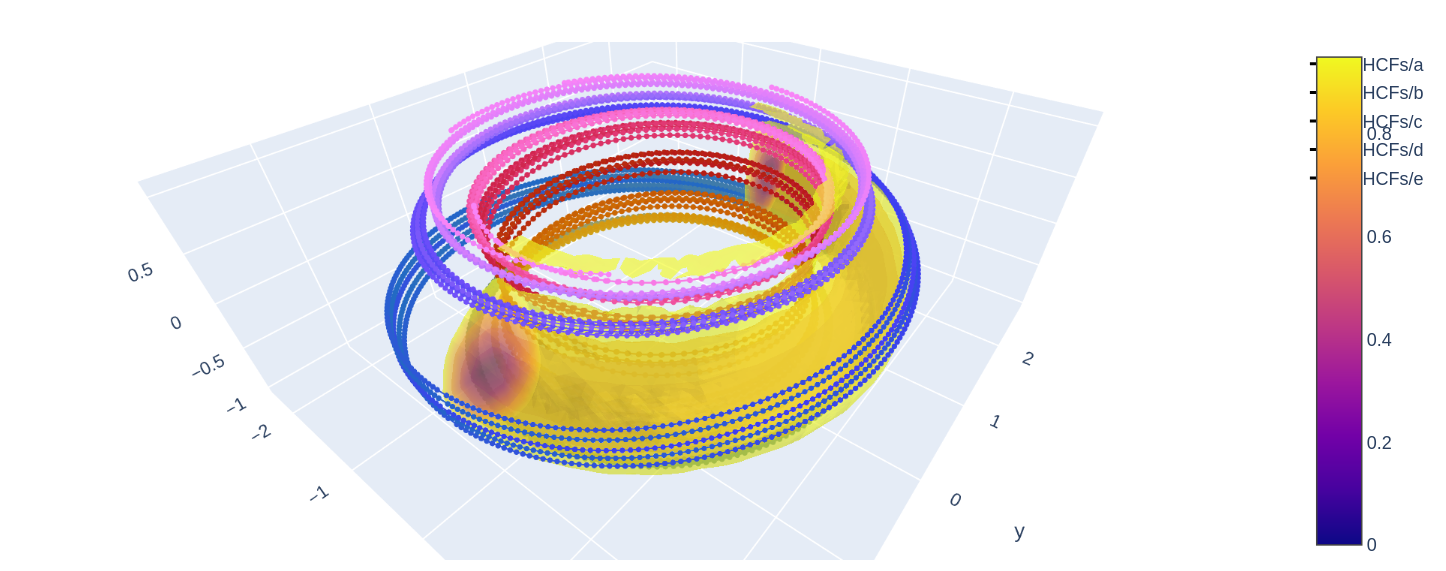
\includegraphics[width=0.47\columnwidth,keepaspectratio]{73999_030400ms_improved/hcfs_east.png}
  }\hfill
  \subcaptionbox{\east 上 RMP 线圈(低 n 线圈)、高 m 线圈及在闭合磁面外 15 mm 余处开始延伸的螺旋电流丝结构图。}{%
  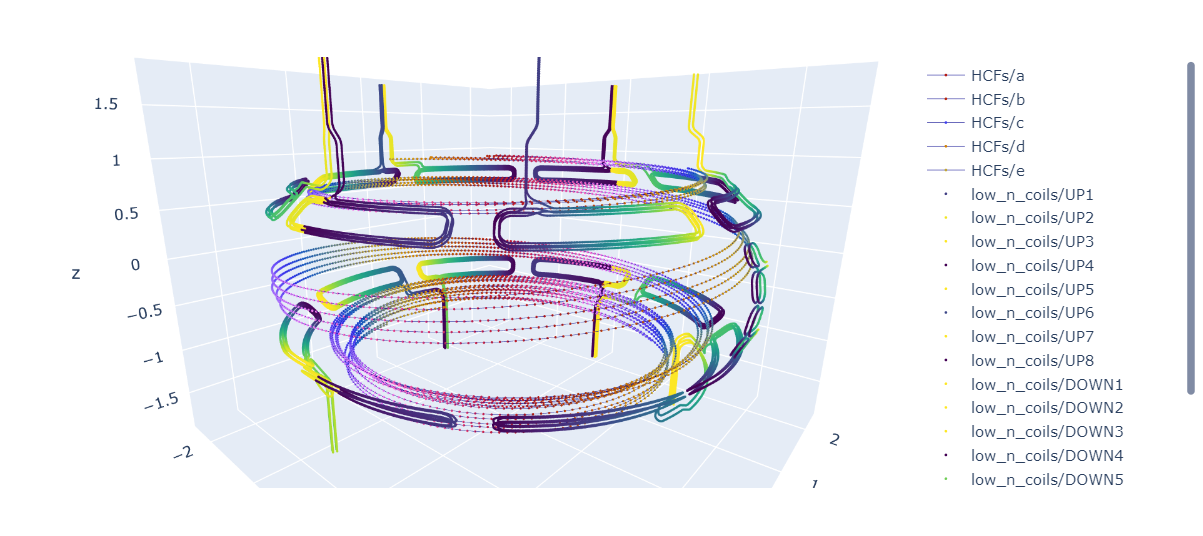
\includegraphics[width=0.47\columnwidth,keepaspectratio]{visual_coilsys.png}
}
\end{figure}

  傅里叶变换的线性性、平移性大大减少了计算磁谱的成本。

  电流强度的变化利用线性性。
  高 m 线圈在 $\varphi$ 正方向上进行移动 $\Delta \varphi$,相当于$\tilde{b}_{m n}^{1}(s)$乘因子 $e^{-i\left(n \Delta\varphi \right )}$。

  下表罗列除了线圈电流幅值、相位及线圈位置等可调参数的可选空间。

  
\begin{table}[htb]
  \centering
  \caption{扰动场可调参量}
  \label{tab:east_parameter}
  \begin{tabularx}{\linewidth}{lXX}
      \toprule[1.5pt]
      变量 & 备注 & 可选区域 \\
      \midrule[1pt]
      $I_{amp~\text{UP}}$ & RMP 线圈上沿电流幅值 & $[-10 \text{kAt}, 10 \text{kAt}]$\\ 
      $I_{amp~\text{DOWN}}$ & RMP 线圈下沿电流幅值 & $[-10 \text{kAt}, 10 \text{kAt}]$\\ 
      $I_{amp~\text{high m, UP}}$ & 高 $m$ 线圈上沿电流幅值 & $[-10 \text{kAt}, 10 \text{kAt}]$\\
      $I_{amp~\text{high m, DOWN}}$ & 高 $m$ 线圈下沿电流幅值 & $[-10 \text{kAt}, 10 \text{kAt}]$\\
      $\Phi_{UP}$ & RMP 线圈上沿电流相位 & $[-\pi, \pi]$\\
      $\Phi_{DOWN}$ & RMP 线圈下沿电流相位 & $[-\pi, \pi]$\\
      $\phi_{\text{high m}}$ & 高 m 线圈环向分布角 & $[-\pi, \pi]$\\
      \bottomrule[1.5pt]
  \end{tabularx}
\end{table}
  

  \begin{itemize}
    \item UP、DOWN 对应的 RMP(Low n) 线圈相位反映的是不同线圈的强度的变化,利用傅里叶变换的线性性减少计算量。
    \item 高 m 线圈的角度是其自身物理位置在柱坐标系统沿中心轴进行环向上的旋转,在 $(\theta^*, \varphi)$ 上沿着 $\varphi$ 平移,利用傅里叶变换的平移性质,相当于$\tilde{b}_{m n}^{1}(s)$乘因子 $e^{-i\left(n \Delta\varphi \right )}$。
    \item 螺旋电流丝的电流强度和位置实验上不太好控制,暂时将其作为给定量。让其他线圈配合它,不让它配合其他线圈。 
  \end{itemize}  
  


\subsection{优化函数}

    
    这是偏工程方面的优化问题,目标函数有两个条件(\Romannum{1})在边界共振分量较大为好(\Romannum{2})在芯部共振分量较小为好,减弱 2/1, 3/1 有理面存在的不稳定性反馈。
    
  品质因子定义 (figure of merit, FoM) $M=\left[\frac{\langle\sigma\rangle_{\psi_{1}<\psi<\psi_{2}}^{4}}{\left\langle\sum_{m, n(n \neq 0)}\left[b_{m n}^{r}\right]^{2}\right\rangle_{\psi_{3}<\psi<\psi_{4}}}\right]$
    
  优化函数的影响指标
  \begin{enumerate}
    \item 越在边界产生的共振分量越重要,积分权重与到有理面共振线的距离成反比 $d=dist(point(n,m),q(\Psi_{pol})n)\downarrow, \rho(m,n,q) \uparrow$。
    \item 减去或除去芯部有理面的共振分量,即其对优化函数呈负贡献。
  \end{enumerate}
    
  \begin{equation}
    \int_{\Psi_{pol}>0.87} \sum_{m,n} \rho(m,n,q) |B_{mn}^r| S(\Psi_{pol})d\Psi_{pol} - \sum_{internal~\Psi_{pol}} \sum_{m,n} \rho(m,n,q) |B_{mn}^r|
  \end{equation}
  
  确定了优化函数后通过共轭梯度法找到一个较优解,或者算力允许的话画等位图。
  
    
  取磁面坐标$(s=\Psi^{1/2}_{pol},\theta^*,\varphi)$,


    
\begin{itemize}
    \item plotly.Isosurface 要求比较规整的数据,非结构数据可能处理不了就不处理了。为了让它能够处理,我进行了插值操作
    \item Field Line Tracing 上周准备了插值和 ODE 的程序工具(Runge-Kutta 5 order),这周已经可以产生迹线了(2D+3D)。
    \item scipy.optimize.minimize 函数作出磁面坐标的归一化半径等高线图。
\end{itemize}

\begin{figure}[htbp]
    \centering%
        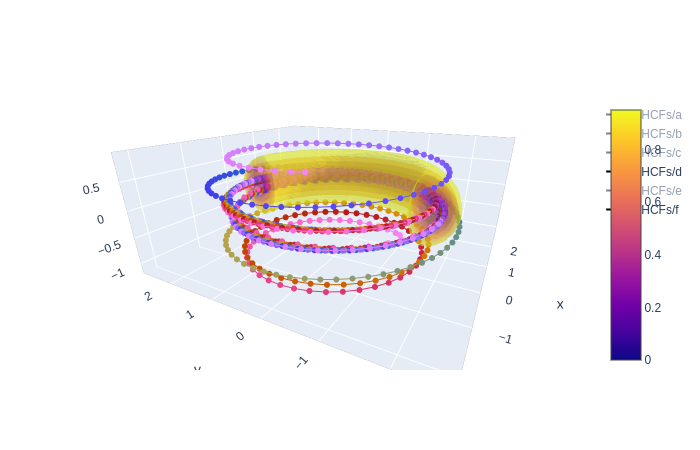
\includegraphics[width=0.95\columnwidth]{magnetic_surface.png}
        \caption{归一化磁面半径为分布在 0 到 0.95 的五个磁面 + 两条磁力线追踪一条在磁力线内,一条在磁力线外。在内可以做 \Poincare 图,在外可以做电流丝。}
\end{figure}

\begin{figure}[htbp]
    \centering%
        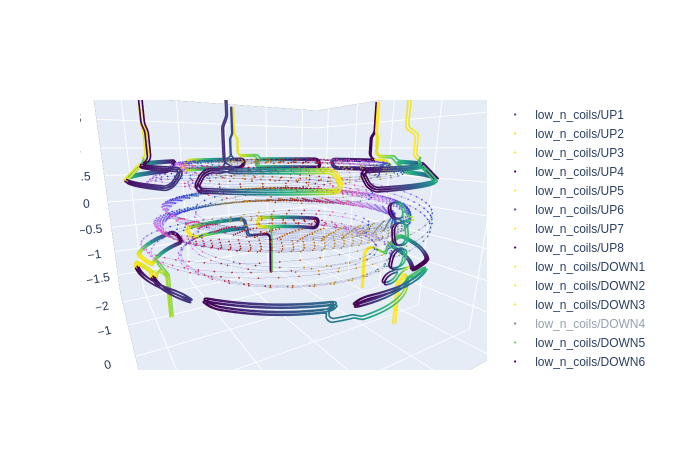
\includegraphics[width=0.95\columnwidth]{coil_collab.png}
        \caption{涉及到的扰动场源的几何形状}
\end{figure}
  
\section{ERGOS 重构}

基于以下几点对 ERGOS 的考虑,本课题进行过程中对磁谱分析程序进行了完全的重建。

ERGOS 计算流程如下:
给定线圈 $\rightarrow$ 计算指定线圈在真空中产生的磁场柱坐标分量 $\underrightarrow{+equilibrium}$  计算磁面坐标系 $\rightarrow$ 计算类径向(radial-like)分量分布 $\rightarrow$ 计算谱图 $\rightarrow$ 其他处理。


在熟悉了 ERGOS 涉及计算的部分之后,受限于 ERGOS 本身的问题 Matlab 诸多函数直接将变量储存于环境中,不太便于函数调用。进行了重构为 Python 的工作。另一方面便于函数封装和并行处理,且检验了原有公式的正确性。

    
  扰动场的截面沿环向扫描,做成动画。
  简化 Merit 变量的程序描述。
\begin{itemize}
  \item ERGOS 原本对每个线圈计算场都要单独写程序。\\
  (a) 统一接口直接处理 Excel 表 (b) 线程并行化和数据复用(网格参数不变即可复用)
    \begin{itemize}
    \item 函数在柱坐标系的分布插值到磁面坐标系上
    \item 磁面坐标系上函数的 fft
    \item chirikov 参数计算
    \item 优化函数计算 figure of merit
    \item 磁面坐标系上的变量分布热力图示意
    \end{itemize}
\end{itemize}

\begin{itemize}
  \item ERGOS 计算 Chrikov 参数的变量依赖于给定的 $n$, 在没有主导的 $n$ 的条件下或者用户给定的 $n$ 不准确的情况下,Chrikov 参数可能是不准确的。
  \item 计算 Merit 时,只考虑了单个 $n$, 可能是当时受限于计算能力。
\end{itemize}

编写了螺旋电流丝沿磁力线运动的程序,并将其保存为线圈一样的表格格式。该程序另一方面在以后的第一壁载荷优化问题中可以再进行拓展。


直接根据扰动场线圈 XYZ 点集工程数据并行计算场分量,改变了原有 ERGOS 需要对每个线圈进行磁场程序单独编写的工作,并且能够充分利用 CPU 。添加了方便的坐标变换函数,减少了日后其他科研人员需要产生磁场数据的工作量。


\begin{itemize}
  \item Field Line Tracing 准备了插值和 ODE 的程序工具(Runge-Kutta 5 order),可以产生迹线了(2D+3D),并且切换其他 ODE 数值计算方法相当方便。原有的 ERGOS FLT 似乎只能在磁面坐标系内进行 FLT,依据柱坐标进行重写之后可以在闭合磁面外追踪。
  \item 2D/3D 作出磁面坐标归一化半径 $s$ 等高线图 2D contour / 3D mesh。
\end{itemize}


  



  
    

\begin{figure}[htbp]
    \centering%
        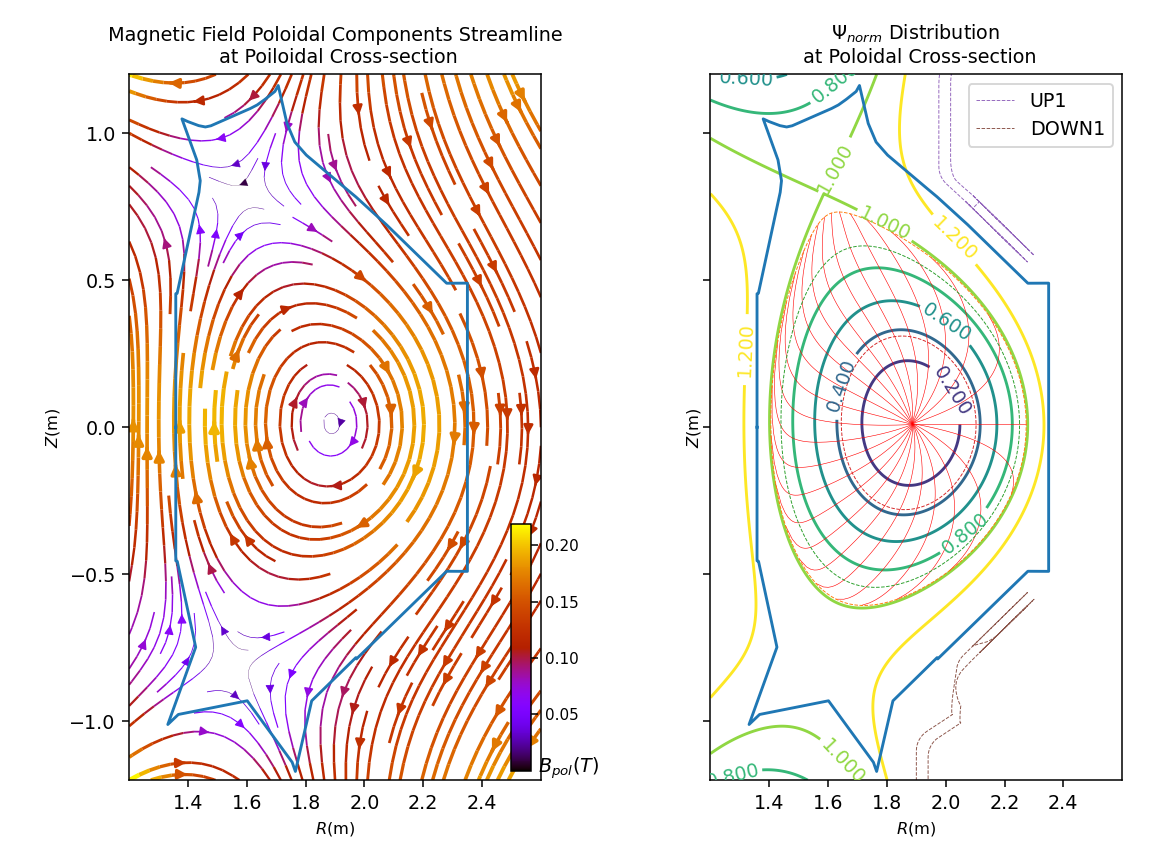
\includegraphics[width=1.00\columnwidth]{pol/pol.png}
        \caption{左图为极向磁面磁场向量流图,右图为 $\Psi_{norm}=s^2$ 分布,右图中还有 RMP 线圈的 UP1、DOWN1 线圈在 RZ 平面的投影。}
\end{figure}



  \begin{figure}[htbp]
      \centering%
          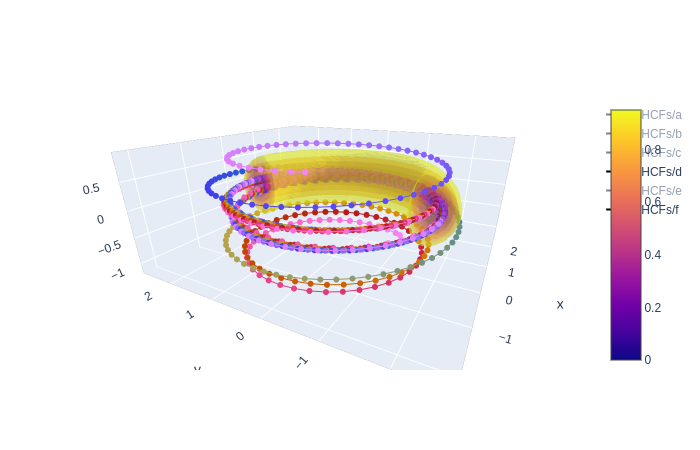
\includegraphics[width=0.95\columnwidth]{magnetic_surface.png}
          \caption{$s$ 分布在 0 到 0.95 的五个磁面, 两条磁力线追踪一条在磁力线内,一条在磁力线外。在内可以做 \Poincare 图,在外可以做电流丝。}
  \end{figure}
  



\section{扰动场协同模拟结果}
在协同模拟实验中,各扰动场在对应的场源为 \SI{1}{\kilo\ampere t} 时的扰动场被保存为场数据文件。标记各扰动场源正方向,\textit{(1) RMP 线圈 / 低 n 线圈} 产生的 $B^1$ 在作用的核心区为正即为正  \textit{(2) 高 m 线圈} 未确定正方向 \textit{(3) HCFs} FLT 电流沿磁场方向即为正方向

\subsection{三者扰动场共同作用}
  当首次进行实验时使三种扰动场同时加入到计算中中发现的一些问题。

  \begin{enumerate}
    \item 对于单边 Single-Null 的位型,上下两侧扰动场线圈产生的扰动场大小明显不同,使得电流相对大小参与到优化中更有必要。
    \item 近期磁谱优化的试验发现,磁谱 $\tilde{b}^1_{mn}$ 的脊线和磁面安全因子对应的曲线贴合程度不足,HCFs 产生的磁场作为基底磁场的影响过大。下一页还有分析。
    \item HCFs 基底磁场对应的 figure of Merit 已经达到 $3.56 * 10^7$, 优化后可以达到 $4.11 * 10^7$,但倍增的系数不大,意义不是很明显,RMP 线圈没有怎么发挥作用。令人吃惊的是不合适地选取 RMP 和 高 m 线圈的各项参数可能导致该值降到 $10^5$ 的量级。 
  \end{enumerate}
  


  





  \begin{figure}[t]
    \centering
    \subcaptionbox{三种线圈共同优化后的结果,在 EAST 73999 Shot 上的 $\tilde{b}^1_{m,n=-2}$ 的绝对值分布。}{%
      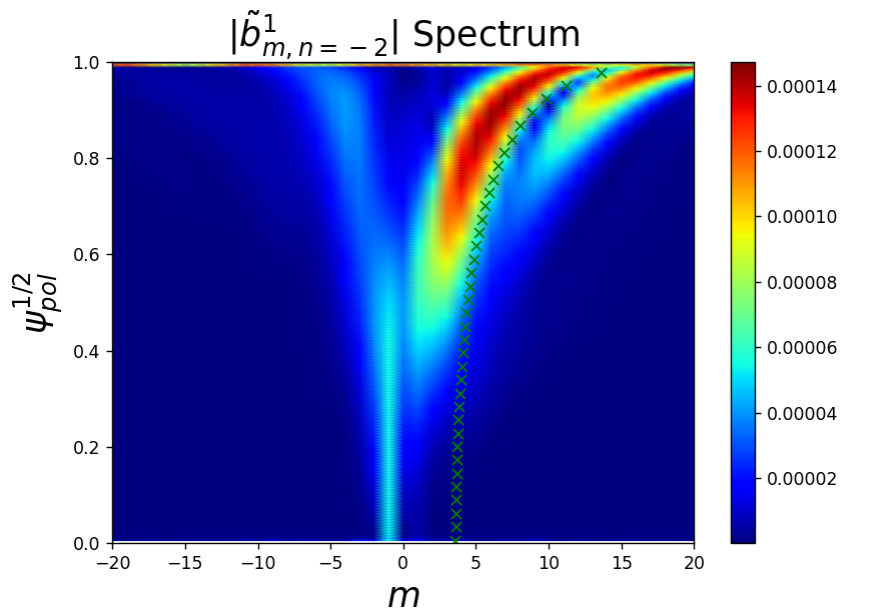
\includegraphics[width=0.47\columnwidth,keepaspectratio]{collab/collab_n=-2_b_sm_nfix_abs.PNG}
    }\hfill
    \subcaptionbox{三种线圈共同优化后的结果,在 EAST 73999 Shot 上的 $\tilde{b}^1_{m,n=-2}$ 的相位分布。}{%
      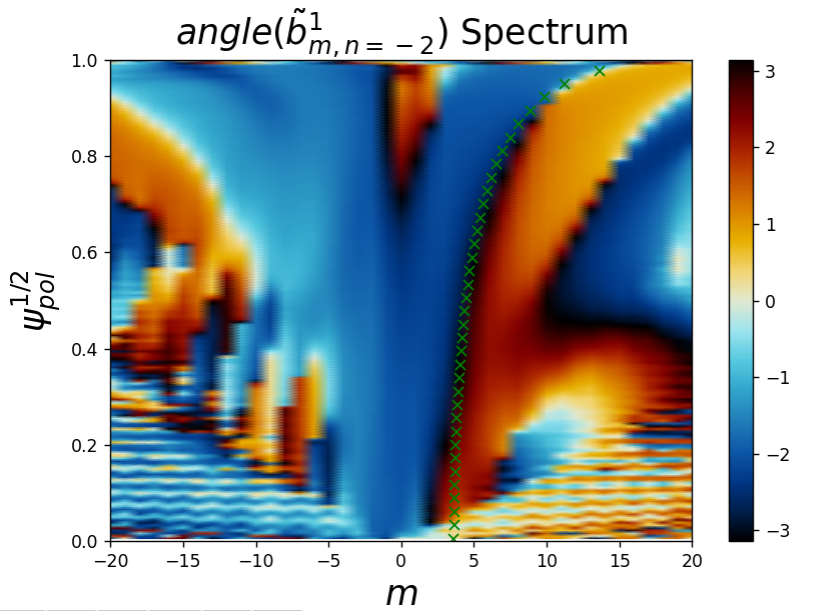
\includegraphics[width=0.47\columnwidth,keepaspectratio]{collab/collab_n=-2_b_sm_nfix_angle.PNG}
    }%
  \end{figure}
  


  
  一开始尝试通过 python 科学计算库 scipy.optimize 函数进行优化得到极值, 但结果中 RMP 线圈的电流值常常在 1 kAt 以下,但高 m 线圈倒是较大,起始以为是陷入了局部极值,随后用了全局随机遍历发现得到的最大值,其对应的磁谱也与上面计算的结果类似,且 RMP 线圈优化得到的电流仍然小于 1 kAt。
  
  

  \begin{figure}[t]
    \centering
    \subcaptionbox{两种线圈共同优化后的结果,在 EAST 73999 Shot 上的 $\tilde{b}^1_{m,n=-2}$ 的绝对值分布。}{%
      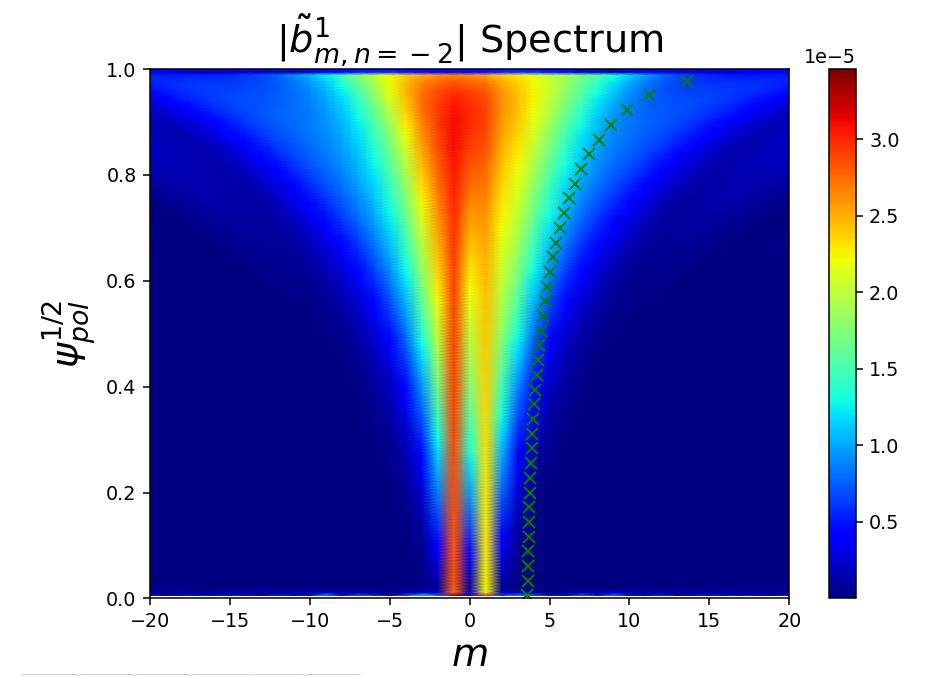
\includegraphics[width=0.47\columnwidth,keepaspectratio]{collab/collab_noHCFs_n=-2_b_sm_nfix_abs.PNG}
    }\hfill
    \subcaptionbox{两种线圈共同优化后的结果,在 EAST 73999 Shot 上的 $\tilde{b}^1_{m,n=-2}$ 的相位分布。}{%
      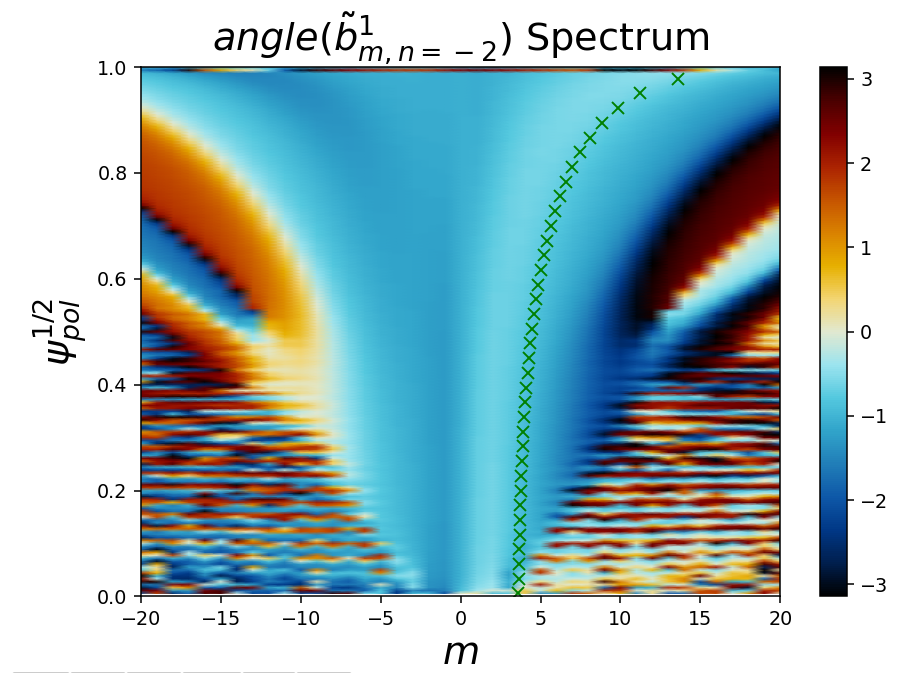
\includegraphics[width=0.47\columnwidth,keepaspectratio]{collab/collab_noHCFs_n=-2_b_sm_nfix_angle.PNG}
    }%
  \end{figure}
  
  随机得到的优化值中 RMP 线圈的电流值在 0.1 kAt 以下(高 m 线圈 -9.01486676 kAt),真是非常有趣。
  
  
  
\begin{figure}[t]
\centering
\subcaptionbox{RMP UP 线圈 kAt 数 - FoM 散点图}{
    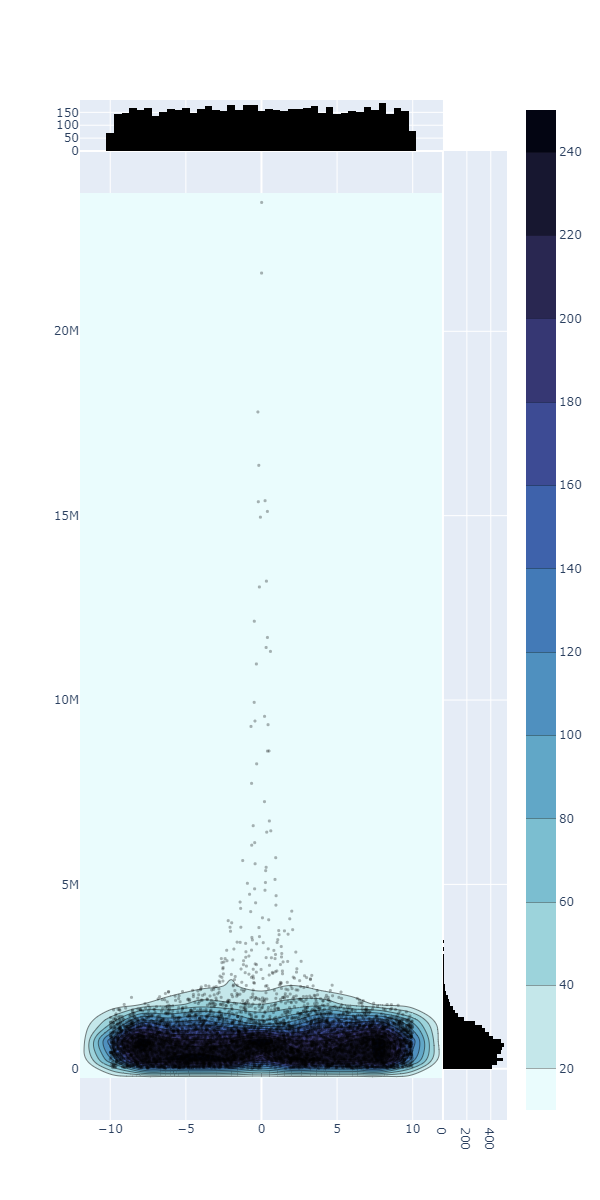
\includegraphics[width=0.32\columnwidth,keepaspectratio]{collab/low_n_UP_FoM.png}
}%\hfill
\subcaptionbox{RMP DOWN 线圈 kAt 数 - FoM 散点图}{
    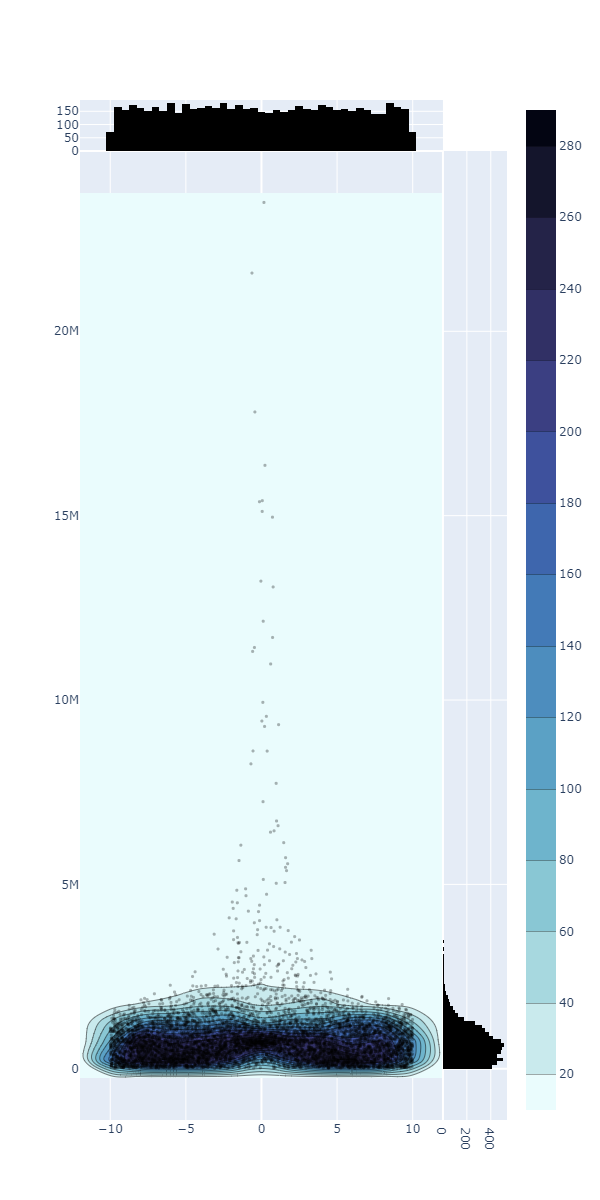
\includegraphics[width=0.32\columnwidth,keepaspectratio]{collab/low_n_DOWN_FoM.png}
}%\hfill
\subcaptionbox{高 m 线圈 kAt 数 - FoM 散点图}{
    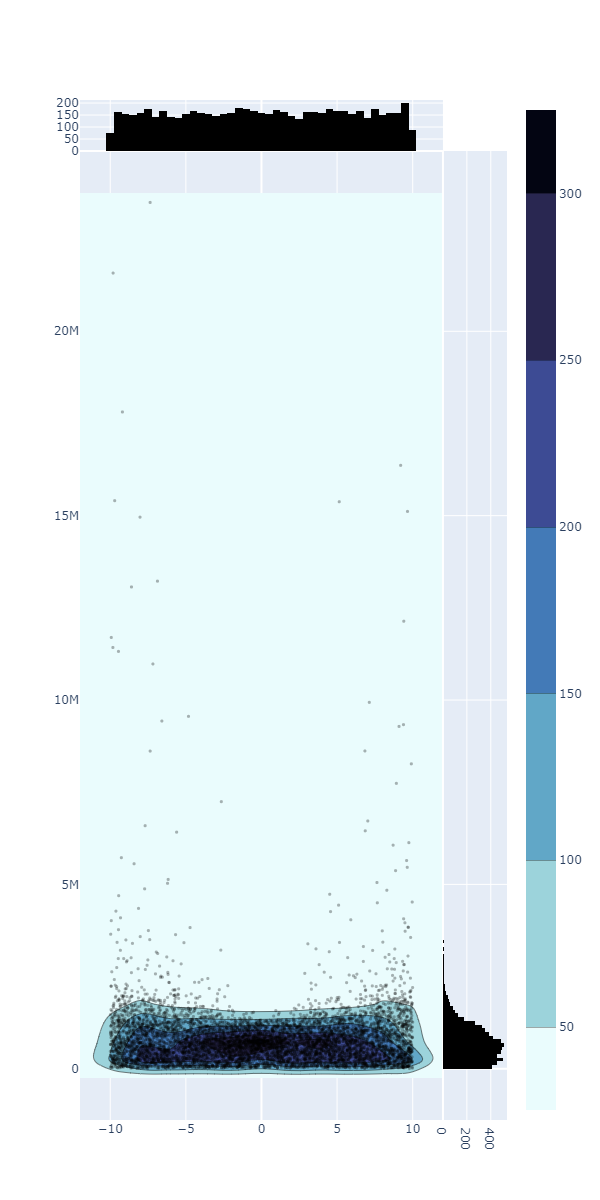
\includegraphics[width=0.32\columnwidth,keepaspectratio]{collab/high_m_FoM.png}
}
\end{figure}
  
  

线圈电流参数对 FoM 的影响参见上面几幅图,明显地有着 kAt 数较低 RMP 线圈和较高 kAt 数的高 m 线圈配合有可能产生较高的 FoM 的趋势,。RMP 线圈相位及高 m 线圈旋转角度三者作为坐标轴后作类似上图,未发现明显变化趋势。
  

高 m 线圈的电流幅度的增大会导致高 FoM 时 RMP 线圈的电流幅值容许范围得以增大。
  
  
\begin{figure}[htbp]
  \centering%
      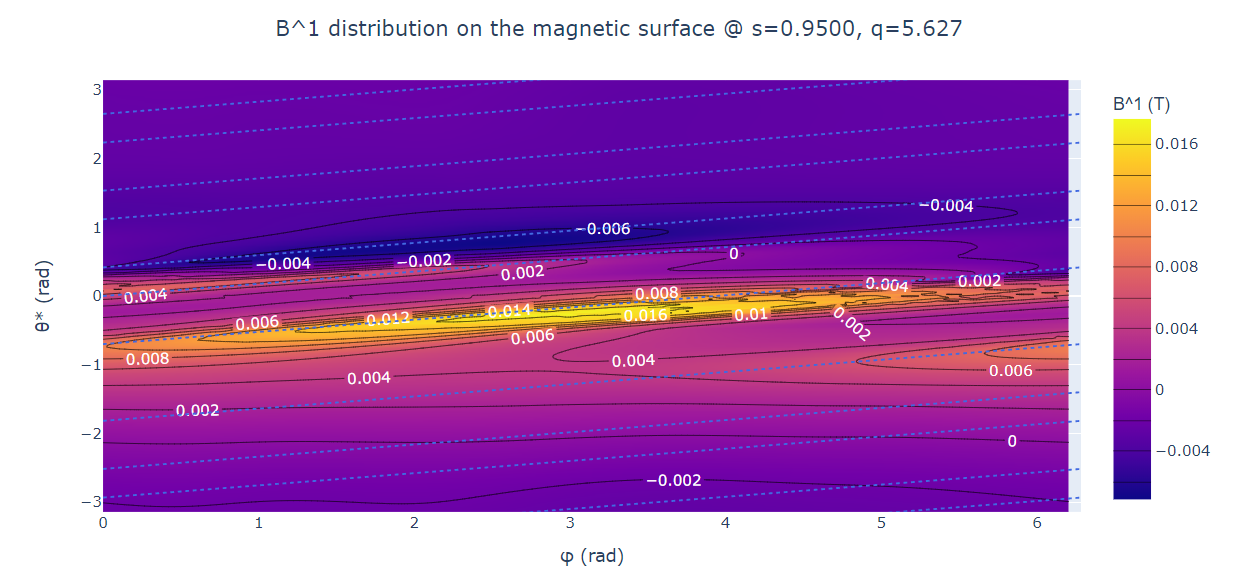
\includegraphics[width=1.0\columnwidth]{hcf/HCFs_uniform.png}
      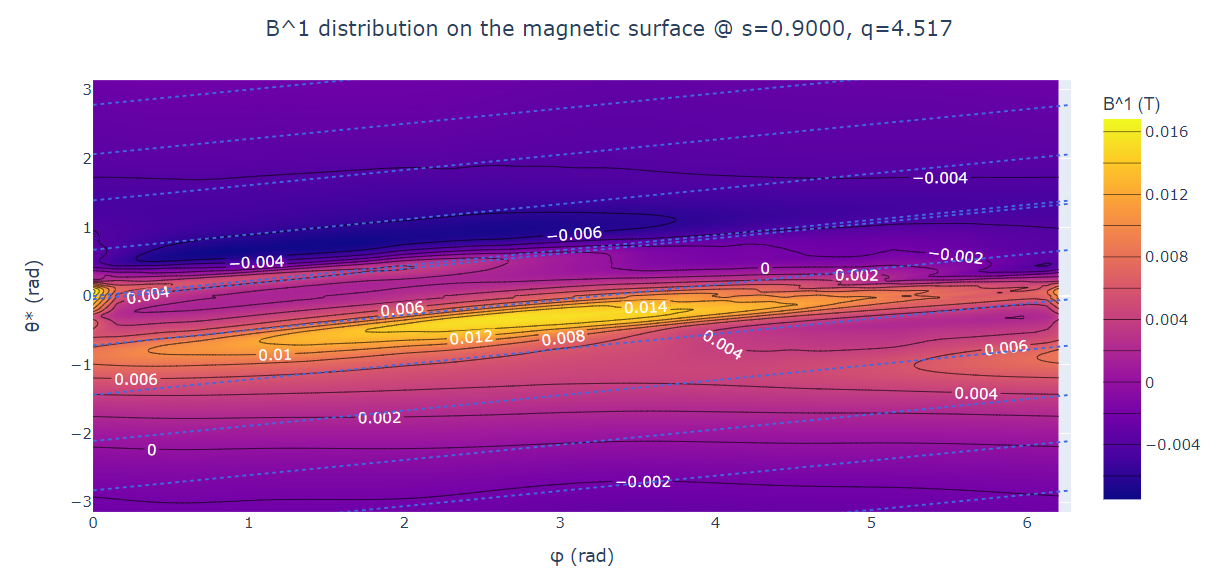
\includegraphics[width=1.0\columnwidth]{collab/collab_n=-2.PNG}
      \caption{上下图分别为 HCFs 产生的基底磁场和三种扰动场优化后的磁场,各自的 $B^1$ 在磁面上 $s=0.950,0.900$ 的分布。虽然没有控制在一个磁面上,但可见优化后对磁场的影响并不大。}
\end{figure}
  
  \begin{itemize}
    \item HCFs 产生的磁场太强,忽略它产生的基底磁场重新测试或者增大 RMP、高 m 线圈电流幅值允许范围。
    \item 在 HCFs 的影响下,磁谱脊线并没有向磁面螺旋度对应的曲线靠拢,反倒是原本的脊线最高值变得更高了。 
  \end{itemize}


在上述的问题出现之后,把螺旋电流丝搁置,暂时先研究低 n (RMP) 线圈和高 m 线圈。


\subsection{RMP 线圈与高 $m$ 线圈扰动场共同作用}
随机得到的优化值中 RMP 线圈的电流值在 0.1 kAt 以下(高 m 线圈 -9.01486676 kAt),虽然可以称为有趣,但作为结果来说是相当糟糕的。
  
\begin{figure}[htbp]
  \centering%
      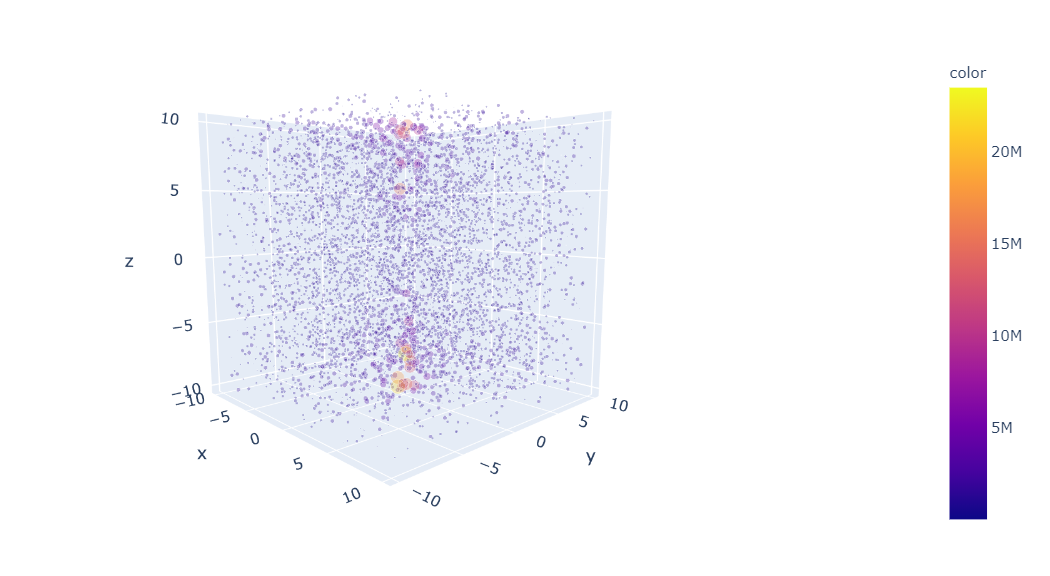
\includegraphics[width=0.45\columnwidth]{collab/Amp_Scatter.png}
      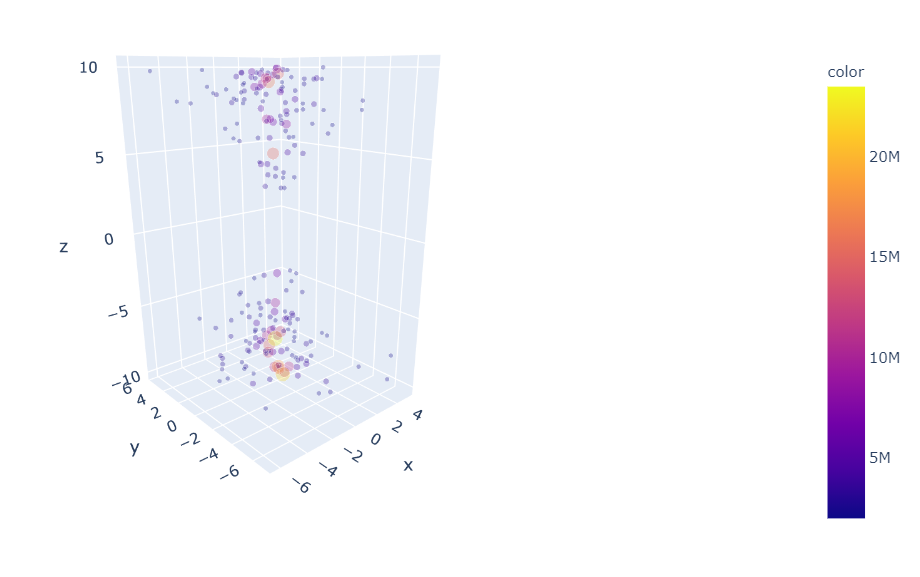
\includegraphics[width=0.45\columnwidth]{collab/Amp_Scatter_FoMthr_2e6.png}
      \caption{左右图均为 RMP 线圈和高 m 线圈进行协同优化后得到的 FoM 分布,marker 的大小和颜色表示 FoM 的大小,坐标轴 XYZ 轴分别为 RMP 线圈上下侧的 电流强度和高 m 线圈的电流强度。右图中过滤去除了 FoM 在 2e6 以下的点。}
\end{figure}

  线圈电流参数对 FoM 的影响参见上面几幅图,明显地有着 kAt 数较低 RMP 线圈和较高 kAt 数的高 m 线圈配合有可能产生较高的 FoM 的趋势,。RMP 线圈相位及高 m 线圈旋转角度三者作为坐标轴后作类似上图,未发现明显变化趋势。
  \begin{itemize}
    \item 高 m 线圈的电流幅度的增大会导致高 FoM 时 RMP 线圈的电流幅值容许范围得以增大。这告诉我们扰动场的大小要匹配(可以用磁通来衡量扰动场的大小)。
  \end{itemize}




计算 Merit 中更方便的变量调整,可以灵活地改变控制的线圈。图中 amp\_setup\_list 控制电流幅度的大小,phase\_setup\_list 控制 RMP 线圈相位的变化,rot\_setup\_list 控制高 m 线圈环向角度。

  
  
  


\begin{figure}[htbp]
    \centering%
    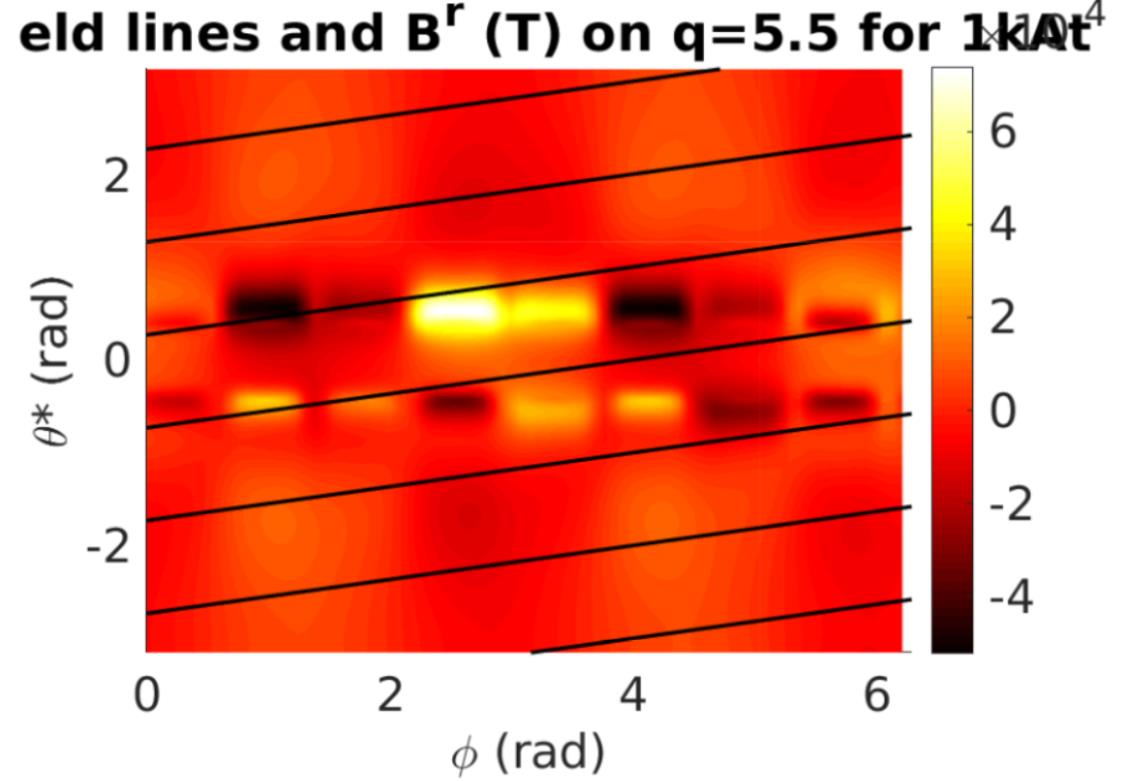
\includegraphics[width=0.85\columnwidth]{Br_flux_surface_q=5_5.jpg}
    \caption{RMP 低 n 线圈工作模式为 Even 时扰动场在 EAST\#73999 $q=5.5$ 磁面上的垂直磁面方向分量的分布。(by ERGOS\cite{nardon_edge_2007})}
\end{figure}




近期将自己编写的磁场输入 ERGOS 进行磁谱计算的试验一方面发现,前期工作还有些问题。从第一次最粗糙的计算来看磁谱 $\tilde{b}^1_{mn}$ 的迹线和各磁面安全因子对应的曲线贴合程度不足。


\begin{figure}[t]
    \centering
    \subcaptionbox{RMP 低 n 线圈工作模式为 Even 时扰动场在 EAST\#73999 $q=5.5$ 磁面上产生的磁谱 $\tilde{b}^1_{mn}$ 。(by ERGOS\cite{nardon_edge_2007})}{%
    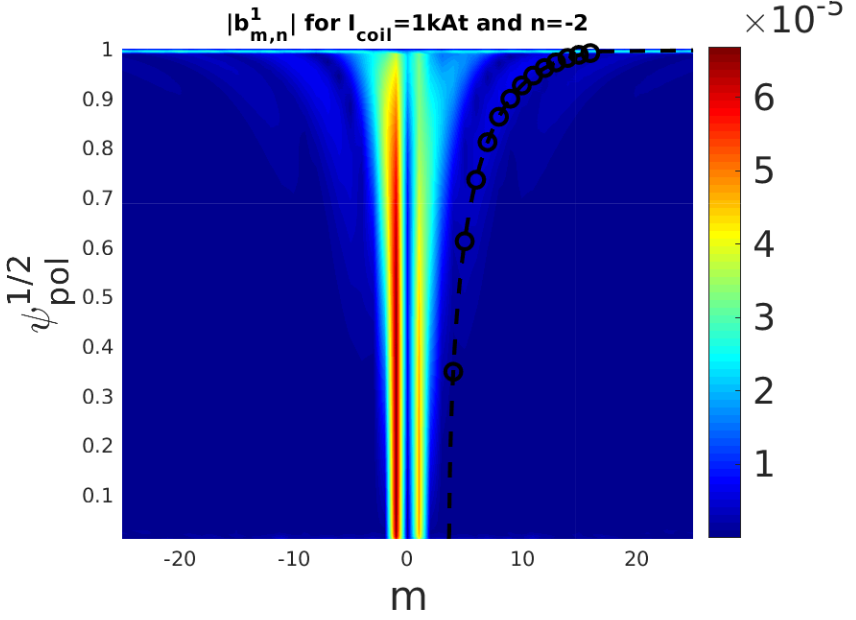
\includegraphics[width=0.35\columnwidth,keepaspectratio]{73999_030400ms_improved/spectrum_1kAt.png}
    }\hfill
    \subcaptionbox{RMP 低 n 线圈各工作模式下下侧线圈电流分布,图中用光滑曲线拟合,实际为阶梯函数。Even 偶连接模式为上下侧线圈没有}{%
    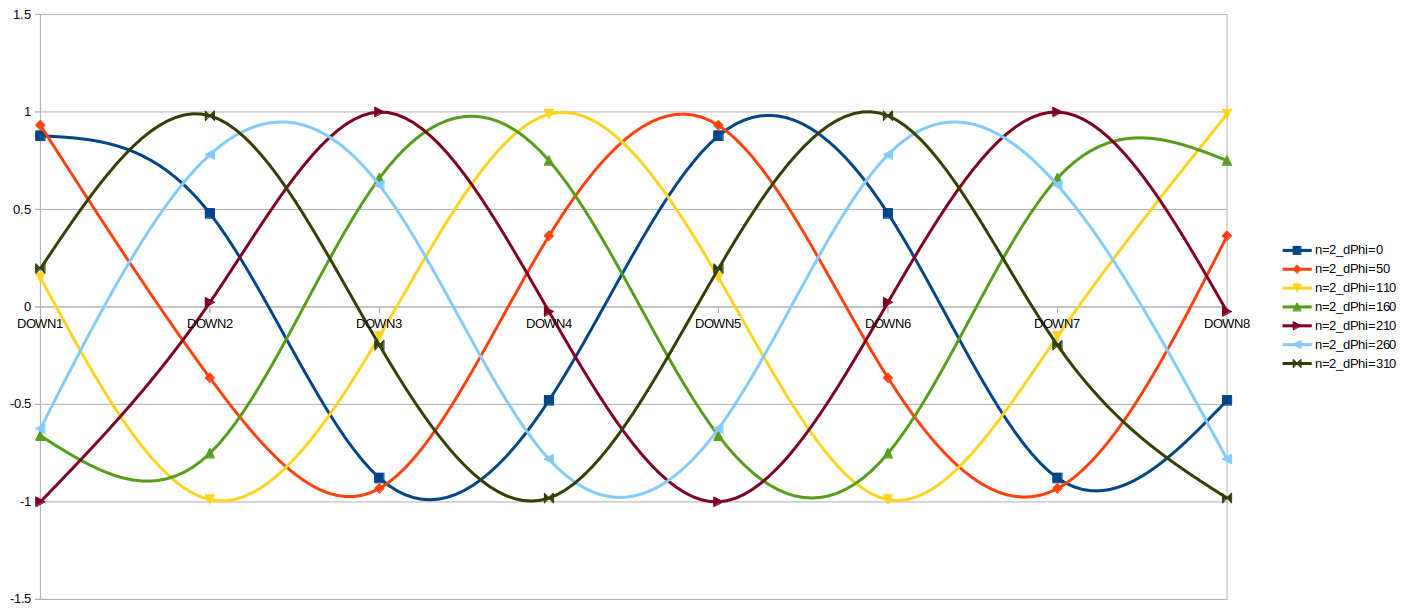
\includegraphics[width=0.6\columnwidth,keepaspectratio]{73999_030400ms_improved/low_n_coils_current.png}
    }%
\end{figure}




  
  
    
  
\begin{itemize}
    \item 程序接口问题,ERGOS Matlab 程序函数作者习惯没有输入输出,变量都是以 Matlab 内部变量储存。
    \item 对角度 $\varphi$ 这种有界参数,优化问题可以做一个扫描。但一旦引入了各扰动场的相对大小,优化方法可能就必需了。但 ERGOS 只适合串行,考虑将 ERGOS 中计算 Chirikov 径向分布计算等部分单独抽出来。FFT 可以不抽出来,因为线性性和平移性对每个线圈做一次计算就可以了。
\end{itemize}
    
扩展多 $n$ 的有理面磁岛半径。

    
  

以下对三种扰动场仿真模拟细节陈述。

% \section{低 n 线圈}

% \subsection{Fourier 分析}

% \subsection{\Poincare 图}
% % \url{https://computing.llnl.gov/projects/starsapphire-data-driven-modeling-analysis/poincar%c3%a9-plots}


% \section{低 n 线圈和螺旋电流丝}

% \subsection{Fourier 分析}

% \subsection{\Poincare 图}

% \section{高 m 线圈、低 n 线圈和螺旋电流丝}

% \subsection{Fourier 分析}

% \subsection{\Poincare 图}
